\section{Lektion 06-02-2018}

\begin{enumerate}
	\item Vinkel modulation
	\item Phasor repræsentation
\end{enumerate}

\begin{mdframed}[style=exampledefault]
	\begin{itemize}
		\item \textbf{Pensum:} JV, Ch 1 p 6-13, p 13-18
		\item \textbf{Opgaver:} P.I-2
	\end{itemize}
\end{mdframed}

\subsection{Vinkel modulation}
Vinkel modulation er processen når frekvensen eller phase af carrieren varrierer i forhold til baseband informationen. Her er amplituden $A_{c0}$ konstant. En vigtig fordel ved PM og FM modulation er at de mere imun overfor channel noise, nonlinear distotion og amplitude fading i forhold til AM modulation. Vinkel modulation kræver en dobbelt så stor båndbredde som AM modulation ($2\cdot W$). \\

\noindent Vinkel modulation er delt op i frekvens (\textbf{FM}) og phase (\textbf{PM}).

\begin{itemize}
	\item Vinkel modulation, $A(t) = A_{c0}$
	\begin{itemize}
		\item \textit{phase modulation, PM} ~\ref{eq:PM}
		\item \textit{frequency modulation, FM} ~\ref{eq:FM}
	\end{itemize}
\end{itemize} 

\begin{equation}\label{eq:PM}
y(t) = A_{c0} \cos(\omega_c t + \beta x(t))
\end{equation}

\begin{equation}\label{eq:FM}
y(t) = A_{c0} \cos(\omega_c t + \phi(t))
\end{equation}

Phase informationen findes ved at differentere.

\begin{equation}\label{eq:FMphi}
\dfrac{d\phi}{dt} = \Delta \omega(t)=\Delta\omega_{max}x(t)=2\pi\Delta f_{max}x(t)
\end{equation}

\begin{description}
	\item[$\beta$] $=\frac{\Delta f_{max}}{f_x}$ maximum phase deviation from the carrier phase
	\item[$\Delta f_{max}$] peak frequency deviation
	\item[$f_x$] baseband frequency component
\end{description}

\textit{The change in phase, changes the frequency of the modulated wave. The frequency of the wave also changes the phase of the wave.}

\begin{figure} [H]
	\centering
	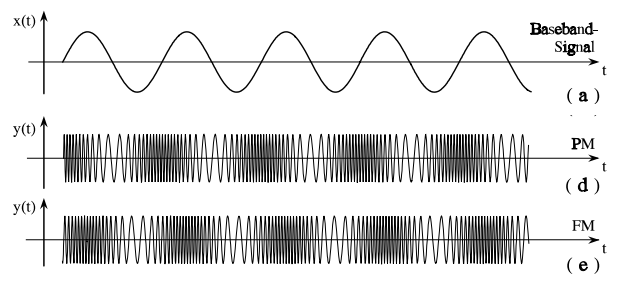
\includegraphics[width=\linewidth]{graphics/8.png}
	\caption{Examples of modulation waveshapes (PM and FM) from a sinusoidal baseband signal $x(t)$.}
	\label{fig:8}
\end{figure}

\subsubsection{PM}
\begin{equation}\label{eq:PM1}
\theta(t) =\omega_c t +\beta x(t)+\phi_0
\end{equation}

\begin{description}
	\item[$x(t)$] Baseband signal
	\item[$\omega_c t$] Angle of Unmodulated carrier wave
	\item[$\beta$]$=\frac{radian}{volt}$ Phase sensitivity (const.)
	\item[$\phi_0$] $=0$ Initial angle
\end{description}

\begin{figure} [H]
	\centering
	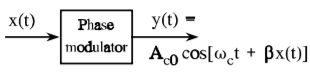
\includegraphics[width=0.5\linewidth]{graphics/10.png}
	\caption{PM angular modulation.}
	\label{fig:10}
\end{figure}

\subsubsection{FM}
\textbf{Indirect FM}
\begin{equation}\label{eq:FM1}
y(t) =A_{c0}\cos[\omega_c t + \beta \int_{}^{} x(t) dt]
\end{equation}

\begin{description}
	\item[$x(t)$] Baseband signal
	\item[$\omega_c t$] Angle of unmodulated carrier wave
	\item[$\beta$]$=\frac{radian}{volt}$ Phase sensitivity (const.)
	\item[$\omega_{inst}$] $=\omega_c + \beta x(t)$ instantaneous frequency.
\end{description}

\begin{figure} [H]
	\centering
	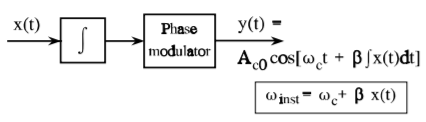
\includegraphics[width=0.65\linewidth]{graphics/11.png}
	\caption{FM indirect modulation.}
	\label{fig:11}
\end{figure}



\noindent\textbf{Direct FM}
\begin{equation}\label{eq:FM2}
y(t) =A_{c0} \cos[\omega_c t +2\pi K_V\int_{}^{} x(t) dt]
\end{equation}

\begin{description}
	\item[$x(t)$] Baseband signal
	\item[$\omega_c t$] Angle of unmodulated carrier wave
	\item[$\beta$]$=\frac{radian}{volt}$ Phase sensitivity (const.)
	\item[$K_V$]$=\frac{hertz}{volt}$ Frequency gain (const.)
	\item[$\omega_{inst}$] $=\omega_c + 2\pi K_V x(t)$ instantaneous frequency.
\end{description}

\begin{figure} [H]
	\centering
	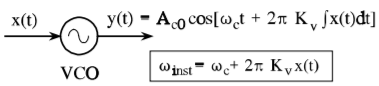
\includegraphics[width=0.65\linewidth]{graphics/12.png}
	\caption{FM direct modulation using VCO.}
	\label{fig:12}
\end{figure}

\subsubsection{Wideband FM}
Tilnærmelsen fra NBFM er ikke gældende ved wideband og derfor gælder følgende. Dette introducerer Bessel funktioner.
\begin{equation}
\cos(\beta_{eff}\sin\omega_x t)=J_0(\beta_{eff})+\sum_{n-2,even}^{\infty}2 J_n(\beta_{eff})\cos n \omega_x t
\end{equation}

\begin{equation}
\sin(\beta_{eff}\sin\omega_x t)=\sum_{n-1,odd}^{\infty}2 J_n(\beta_{eff})\sin n \omega_x t
\end{equation}

\begin{description}
	\item[$\beta_{eff}$] $=\beta A_x$ effective modulation index
	\item[$n_{99\%}$] $\approx \beta_{eff}+1$ 
\end{description}

\begin{figure} [H]
	\centering
	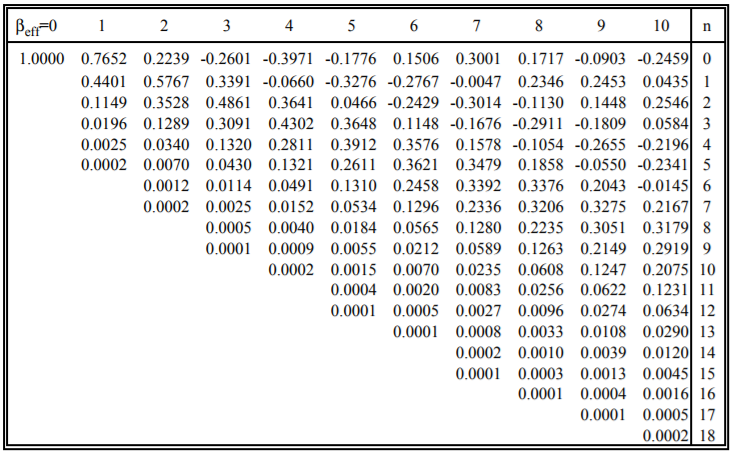
\includegraphics[width=\linewidth]{graphics/13.png}
	\caption{$J_n(\beta_{eff})$, expansion coefficients from Bessel functions.}
	\label{fig:13}
\end{figure}

Bessel funktioner indsættes.

\begin{equation}
y(t)|_{FM or PM} = A_{c0}J_0 (\beta_{eff})\cos(\omega_c t)
\end{equation}

\begin{equation}
y(t)|_{FM or PM} = A_{c0} \sum_{n=-\infty}^{\infty}J_n(\beta_{eff})\cos(\omega_c t+n\omega_x t)
\end{equation}

\newpage\noindent\textbf{Accumalted power}
\begin{equation}
p_{ac,n}(\beta_{eff}) = \dfrac{P_{ac,n}}{\frac{A_{c0}^2}{2}}=J_0^2(\beta_{eff})+\sum_{i=1}^{n}2J_i^2(\beta_{eff})
\end{equation}
\noindent\textbf{Bandwidth for 99\% power}
\begin{itemize}
	\item \textit{phase modulation, PM} ~\ref{eq:ppm}
	\item \textit{frequency modulation, FM} ~\ref{eq:pfm}
\end{itemize}

\begin{equation}\label{eq:ppm}
W_{99\%}=2\omega_x(\beta_{eff}+1)=2\omega_x[\beta A_x+1]
\end{equation}

\begin{equation}\label{eq:pfm}
W_{99\%}=2\omega_x(\beta_{eff}+1)=2[\Delta\omega_{max} A_x+\omega_x]
\end{equation}

\begin{figure} [H]
	\centering
	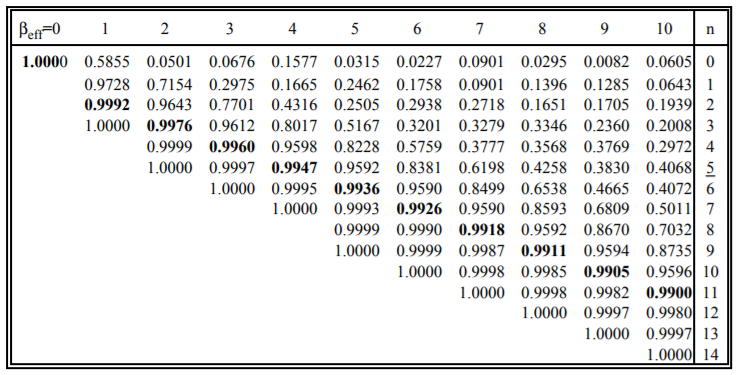
\includegraphics[width=\linewidth]{graphics/14.png}
	\caption{$p_{ac,n}(\beta_{eff})$, accumulated relative power of frequency components to and including	order \textit{n} in size. Figures in bold indicate the first 99\% bound passing.}
	\label{fig:14}
\end{figure}

\subsection{Phasor repræsentation}

\begin{figure} [H]
	\centering
	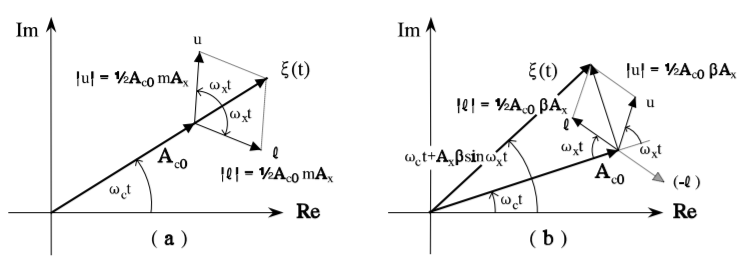
\includegraphics[width=\linewidth]{graphics/9.png}
	\caption{Phasor representation showing how the lower and upper sideband components, \textit{l}	and \textit{u}, add to the carrier $A_{c0}$ in (a) AM modulation, and (b) narrowband FM. The modulated wave becomes $y(t)=Re(\zeta)$.}
	\label{fig:9}
\end{figure}
